\documentclass[aspectratio=169]{../latex_main/tntbeamer}  % you can pass all options of the beamer class, e.g., 'handout' or 'aspectratio=43'
\usepackage{dsfont}
\usepackage{bm}
\usepackage[english]{babel}
\usepackage[T1]{fontenc}
%\usepackage[utf8]{inputenc}
\usepackage{graphicx}
\graphicspath{ {./figures/} }
\usepackage{algorithm}
\usepackage[ruled,vlined,algo2e,linesnumbered]{algorithm2e}
\usepackage{hyperref}
\usepackage{booktabs}
\usepackage{mathtools}

\usepackage{amsmath,amssymb}

\DeclareMathOperator*{\argmax}{arg\,max}
\DeclareMathOperator*{\argmin}{arg\,min}

\usepackage{pgfplots}
\pgfplotsset{compat=1.16}
\usepackage{tikz}
\usetikzlibrary{trees} 
\usetikzlibrary{shapes.geometric}
\usetikzlibrary{positioning,shapes,shadows,arrows,calc,mindmap}
\usetikzlibrary{positioning,fadings,through}
\usetikzlibrary{decorations.pathreplacing}
\usetikzlibrary{intersections}
\pgfdeclarelayer{background}
\pgfdeclarelayer{foreground}
\pgfsetlayers{background,main,foreground}
\tikzstyle{activity}=[rectangle, draw=black, rounded corners, text centered, text width=8em]
\tikzstyle{data}=[rectangle, draw=black, text centered, text width=8em]
\tikzstyle{myarrow}=[->, thick, draw=black]

% Define the layers to draw the diagram
\pgfdeclarelayer{background}
\pgfdeclarelayer{foreground}
\pgfsetlayers{background,main,foreground}

% Requires XeLaTeX or LuaLaTeX
\usepackage{unicode-math}

\usepackage{fontspec}
%\setsansfont{Arial}
\setsansfont{RotisSansSerifStd}[ 
Path=../latex_main/fonts/,
Extension = .otf,
UprightFont = *-Regular,  % or *-Light
BoldFont = *-ExtraBold,  % or *-Bold
ItalicFont = *-Italic
]
\setmonofont{Cascadia Mono}[
Scale=0.8
]

% scale factor adapted; mathrm font added (Benjamin Spitschan @TNT, 2021-06-01)
%\setmathfont[Scale=1.05]{Libertinus Math}
%\setmathrm[Scale=1.05]{Libertinus Math}

% other available math fonts are (not exhaustive)
% Latin Modern Math
% XITS Math
% Libertinus Math
% Asana Math
% Fira Math
% TeX Gyre Pagella Math
% TeX Gyre Bonum Math
% TeX Gyre Schola Math
% TeX Gyre Termes Math

% Literature References
\newcommand{\lit}[2]{\href{#2}{\footnotesize\color{black!60}[#1]}}

%%% Beamer Customization
%----------------------------------------------------------------------
% (Don't) Show sections in frame header. Options: 'sections', 'sections light', empty
\setbeamertemplate{headline}{empty}

% Add header logo for normal frames
\setheaderimage{
	% 
\includegraphics[height=\logoheight]{figures/TNT_darkv4.pdf}
	
\includegraphics[height=\logoheight]{../latex_main/figures/luh_logo_rgb_0_80_155.pdf}
	% 
\includegraphics[height=\logoheight]{figures/logo_tntluh.pdf}
}

% Header logo for title page
\settitleheaderimage{
	% 
\includegraphics[height=\logoheight]{figures/TNT_darkv4.pdf}
	
\includegraphics[height=\logoheight]{../latex_main/figures/luh_logo_rgb_0_80_155.pdf}
	% 
\includegraphics[height=\logoheight]{figures/logo_tntluh.pdf}
}

% Title page: tntdefault 
\setbeamertemplate{title page}[tntdefault]  % or luhstyle
% Add optional title image here
%\addtitlepageimagedefault{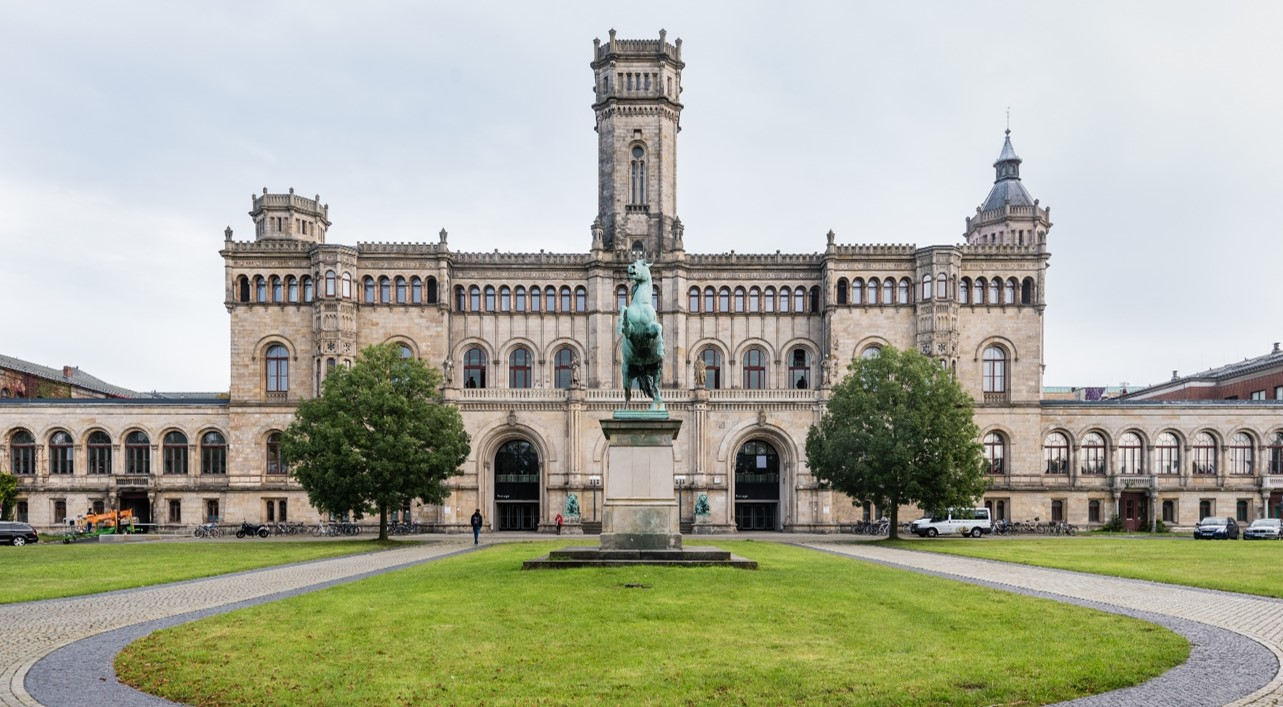
\includegraphics[width=0.65\textwidth]{figures/luh_default_presentation_title_image.jpg}}

% Title page: luhstyle
% \setbeamertemplate{title page}[luhstyle]
% % Add optional title image here
% \addtitlepageimage{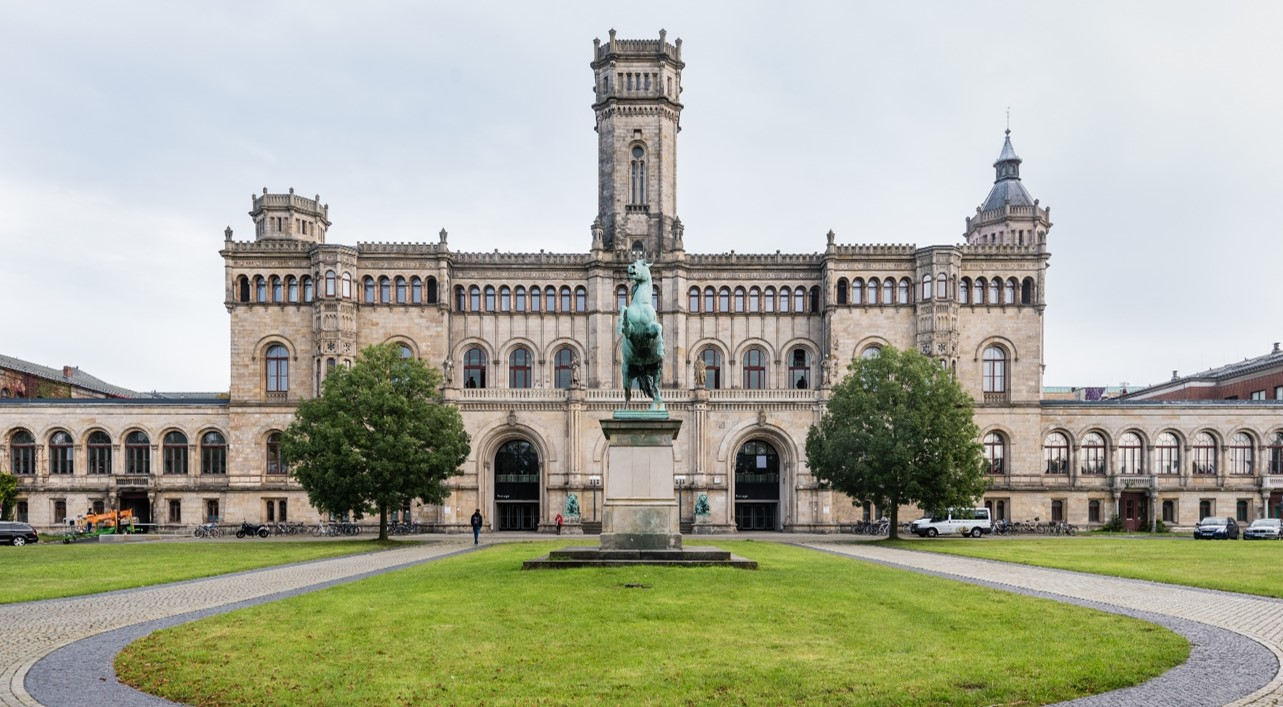
\includegraphics[width=0.75\textwidth]{figures/luh_default_presentation_title_image.jpg}}

\author[Lindauer \& Anand]{Marius Lindauer and Avishek Anand\\[1em]
	
\includegraphics[height=\logoheight]{../latex_main/figures/luh_logo_rgb_0_80_155.pdf}\qquad

\includegraphics[height=\logoheight]{../latex_main/figures/TNT_darkv4}\qquad

\includegraphics[height=\logoheight]{../latex_main/figures/L3S.jpg}	}
\date{Winter Term 2021
}


%%% Custom Packages
%----------------------------------------------------------------------
% Create dummy content
\usepackage{blindtext}

% Adds a frame with the current page layout. Just call \layout inside of a frame.
\usepackage{layout}


\title[Introduction]{iML: Introduction}
\subtitle{Concepts}
%\institute{}

\begin{document}
	
	\maketitle


\begin{frame}[c]{What tools do we have?}
	\begin{center}
		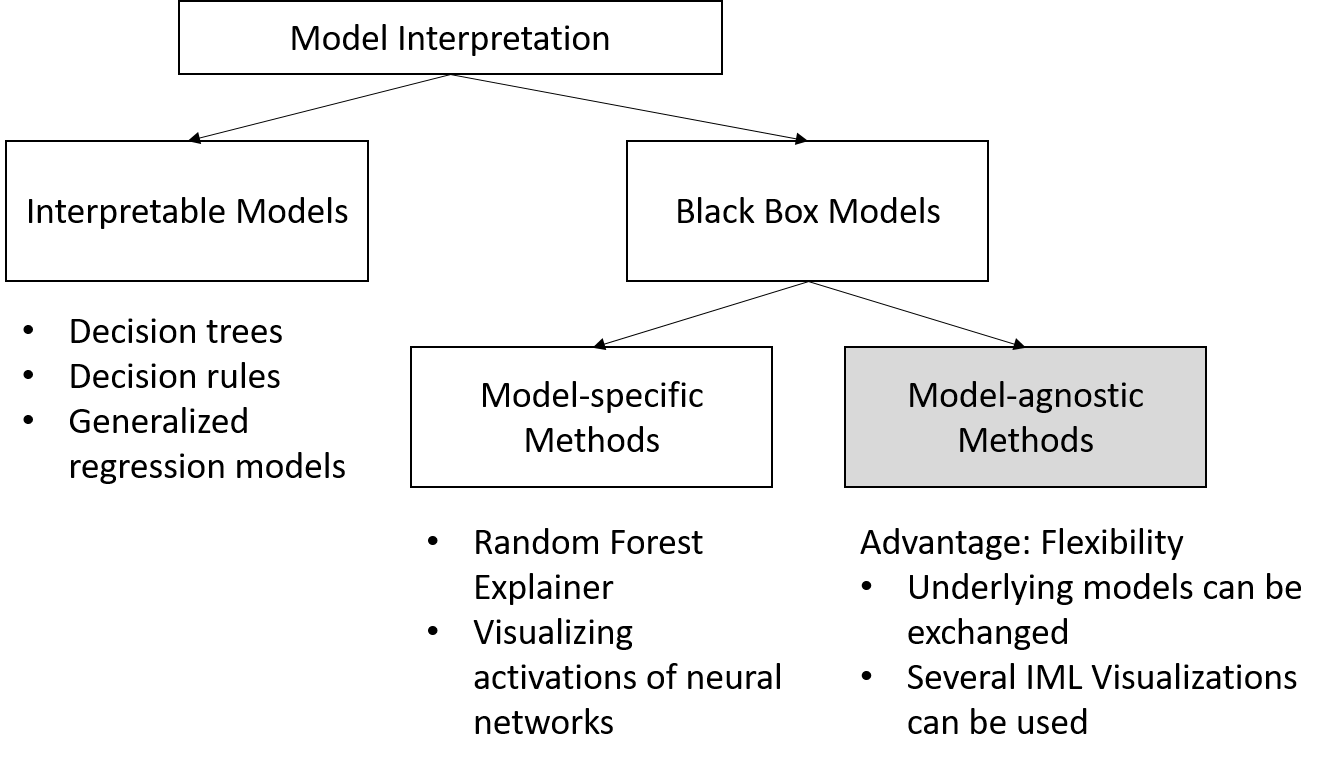
\includegraphics[width=0.7\textwidth]{figure/overview}
	\end{center}
\end{frame}

\begin{frame}[c]{Intrinsic and Model-Agnostic Interpretation}
	\begin{itemize}
		\item Intrinsically interpretable models:
		\begin{itemize}
			\item Examples are linear models and decision trees.
			\item They are interpretable because of their simple structures,\\ 
			e.g. weighted combination of feature values or tree structure. 
			\item They are difficult to interpret with many features or complex interaction terms.
		\end{itemize}
	\bigskip
	\pause
		\item Model-agnostic interpretation methods:
		\begin{itemize}
			\item They are applied after training (post-hoc).
			\item They also work for more complex black box models.
			\item They can also be applied to intrinsically interpretable models,\\ 
			e.g. feature importance for decision trees. 
		\end{itemize}
	\end{itemize}
\end{frame}

\begin{frame}[c]{Model-Agnostic Interpretability}
	\begin{itemize}
		\itemsep2em
		\item Model-agnostic interpretability methods work for \textbf{any} kind of machine learning model.
		\item Explanation type is not tied to the underlying model type.
		\item Often, only access to data and fitted predictor is required.\\
		 No further knowledge about the model itself is necessary.
		\item We usually distinguish between \textbf{feature effect} and \textbf{feature importance} methods.
	\end{itemize}
\end{frame}


\begin{frame}[c]{Feature Effects vs. Feature Importance}
	\vspace{-1em}
	\textbf{Feature Effects} visualize or quantify the (average) relationship or contribution of a feature to the model prediction.
	\begin{center}
		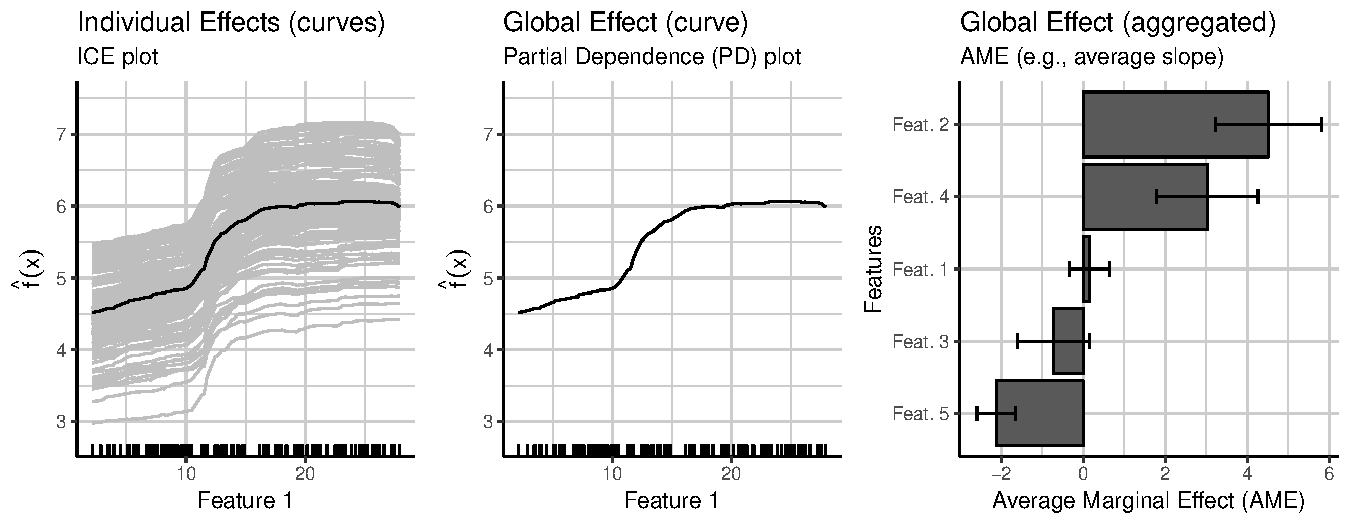
\includegraphics[page=1, width=0.7\textwidth]{figure/feature-effects}
	\end{center}
	\begin{itemize}
		\item Methods: Partial Dependence Plots, Individual Conditional Expectation,\\ Accumulated Local Effects (ALE)
		\item Pendant in linear models: Regression coefficient $\hat{\theta}_j$
	\end{itemize}
\end{frame}

\begin{frame}[c]{Feature Effects vs. Feature Importance (cont'd)}
	
	\textbf{Feature importance} methods rank features by how much they contribute to the predictive performance or prediction variance of the model.
	\begin{columns}
		\begin{column}{0.6\textwidth}
			\begin{itemize}
				\itemsep1em
				\item Methods: Permutation Feature Importance,\\ Functional Anova
				\item Analog in linear models: Absolute t-statistic %$\left|\frac{\hat{\theta}_j}{SE(\hat{\theta}_j)}\right|$
			\end{itemize}
		\end{column}
		\begin{column}{0.4\textwidth}
			\begin{center}
				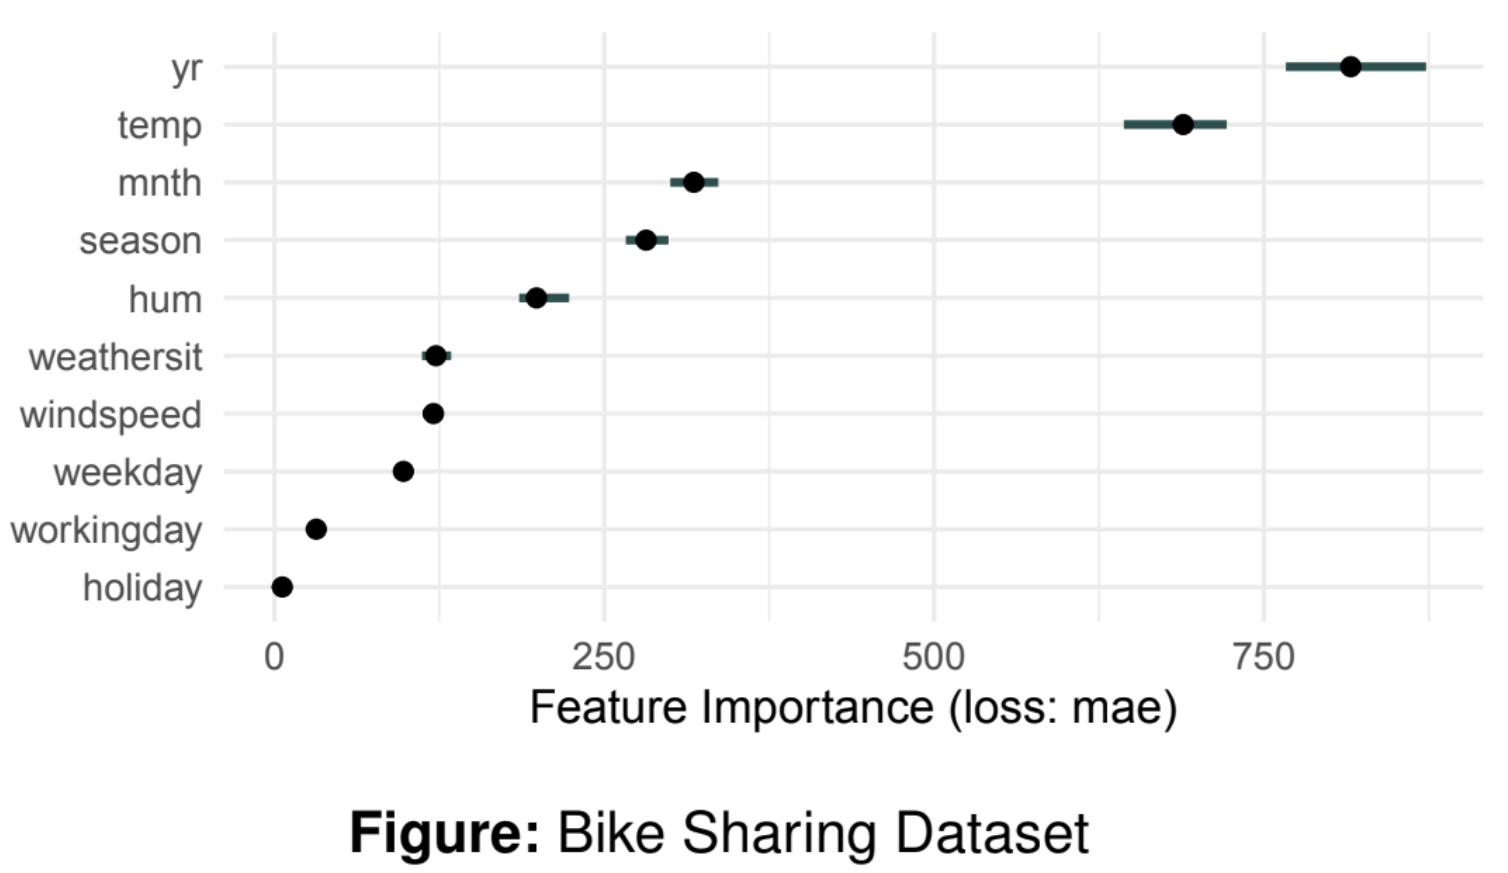
\includegraphics[page=1, width=0.9\textwidth]{figure/feature-importance}
			\end{center}
		\end{column}
	\end{columns}
\end{frame}


\begin{frame}[c]{Global and Local Interpretability}
	Global interpretability methods explain the expected model behavior for the entire input space by considering all available observations (or representative subsets). For example:
	\begin{itemize}
		\item Permutation Feature Importance
		\item Partial Dependence Plot
		\item Functional Anova
		\item ...
	\end{itemize}
	Local interpretability methods explain single predictions or a group of similar observations.\\ For example:
	\begin{itemize}
		\item Individual Conditional Expectation (ICE) Plots
		\item Local Interpretable Model-Agnostic Explanations (LIME)
		\item Shapley Values
		\item ...
	\end{itemize}
\end{frame}


\begin{frame}[c]{Fixed Model vs. Refits}
	\begin{itemize}
		\itemsep1em
		\item Most methods, we will discuss, analyze a fixed, trained model\\ 
		(e.g., permutation feature importance).
		\item Some methods require refitting the model (e.g., PIMP).
		\item Trained model $\Rightarrow$ Model is the object of analysis.
		\item Refitting $\Rightarrow$ Learning process is the object of analysis.
		\item The advantage of refitting is\\ that it includes information about the variability in the learning process.
	\end{itemize}
\end{frame}

	
\end{document}
